\chapter{Orientasi dan Bahasa Bersama Cloud-Native}
\label{ch:ch01-orientasi}

% Kolom rata kiri untuk tabel bab ini, agar spasi antarkata pada kolom sempit tidak
% meregang. L untuk kolom lentur, P untuk kolom dengan lebar tetap.
\newcolumntype{L}{>{\raggedright\arraybackslash}X}
\newcolumntype{P}[1]{>{\raggedright\arraybackslash}p{#1}}

\section*{Tujuan Pembelajaran}
\begin{itemize}
  \item Menjelaskan dengan bahasa sehari-hari istilah dasar sistem informasi: aplikasi,
        server, basis data, jaringan, pusat data, dan \textit{cloud}.
  \item Mengaitkan keputusan teknologi dengan nilai bisnis, biaya, risiko, dan regulasi.
  \item Merumuskan masalah teknologi informasi di organisasi pilihan tim sebagai pemicu
        modernisasi.
\end{itemize}

\section{Pendahuluan}

Rapat direksi Medikara Health, jaringan layanan kesehatan fiktif yang dipakai sepanjang
modul ini, membahas laporan triwulan pertama 2026. Isinya tidak menggembirakan. Antrean
pendaftaran rawat jalan masih panjang, terutama pada Senin pagi. Lima rumah sakit
menjalankan Sistem Informasi Manajemen Rumah Sakit (SIMRS) dengan versi yang
berbeda-beda, sehingga setiap sambungan baru ke mitra harus dibangun lima kali. Biaya
integrasi terus naik. Di akhir rapat, seorang direktur bertanya: "Kalau semua sistem
dipindahkan ke \textit{cloud}, apakah masalah ini selesai?"

Pertanyaan itu wajar dan terdengar di banyak organisasi. Jawabannya tidak sesederhana
"ya" atau "tidak". Antrean bisa disebabkan alur pendaftaran, bukan oleh server. Lima
versi SIMRS tetap lima versi walaupun dipindahkan ke pusat data lain. Biaya integrasi
bahkan bisa naik bila setiap sambungan harus dibangun ulang di tempat baru. Mata kuliah
ini melatih cara menjawab pertanyaan semacam itu dengan runtut: berangkat dari masalah
organisasi, menimbang pilihan beserta \textit{trade-off}-nya, lalu menuliskan
justifikasi yang dapat dipertanggungjawabkan di depan manajemen.

Bab ini menyiapkan tiga bekal. Pertama, cara kerja mata kuliah dan kaitannya dengan
proyek capstone. Kedua, bahasa bersama bagi kelas yang berlatar campuran: istilah dasar
sistem informasi bagi mahasiswa non-teknis, serta istilah nilai bisnis, biaya, dan
risiko bagi mahasiswa teknis. Ketiga, kualitas sistem yang saling tarik-menarik dan
arti \textit{cloud-native} bagi organisasi. Rujukan utamanya adalah definisi
\textit{cloud computing} dari National Institute of Standards and Technology (NIST)
\cite{nist800-145}, definisi \textit{cloud native} dari Cloud Native Computing
Foundation (CNCF) \cite{cncf-definition}, serta pandangan Richards dan Ford bahwa setiap
keputusan arsitektur adalah \textit{trade-off} \cite{richards2025}.

\section{Cara Kerja Mata Kuliah dan Proyek Capstone}

Mata kuliah ini dipelajari secara mandiri lewat modul dan slide. Tatap muka hanya
berlangsung pada hari Sabtu, dan waktunya dipakai untuk membahas progres proyek
capstone, bukan untuk mengulang isi modul. Artinya, setiap bab dibaca sebelum Sabtu,
Aktivitas dikerjakan bersama tim, lalu draf artefaknya dibawa ke kelas untuk ditinjau.
Pola ini mirip bimbingan tugas akhir: pertemuan dengan pembimbing dipakai untuk membahas
draf yang sudah ada, bukan untuk mendengar ceramah. Dengan 8 tim dan tatap muka 150
menit, setiap tim mendapat sekitar 15 menit. Tim yang datang tanpa draf menghabiskan
waktu itu untuk menjelaskan rencana, sehingga umpan baliknya umum dan pekerjaan pekan
berikutnya menumpuk.

\subsection{Empat Mata Kuliah, Satu Cetak Biru}

Mata kuliah IT40713 adalah satu dari empat mata kuliah peminatan Digital Enterprise
Architecture. Keempatnya menyusun satu proyek capstone bersama, yaitu Cetak Biru
Transformasi Digital untuk satu organisasi. Gambar \ref{fig:ch01-capstone}
memperlihatkan pembagian tugasnya. IT40513 Enterprise Architecture \& Digital Blueprint
menyusun \textit{capability map}, arsitektur bisnis, dan arsitektur aplikasi. IT40613
Digital Platform \& API Economy merancang platform dan Application Programming Interface
(API) untuk ekosistem mitra. IT40813 IT Governance, Risk \& Compliance menyusun tata
kelola, daftar risiko, dan kepatuhan. IT40713 bertanggung jawab atas strategi
\textit{cloud}, penilaian portofolio aplikasi, arsitektur target berbasis
\textit{cloud-native}, serta rencana operasi dan modernisasinya.

\begin{figure}[!htb]
  \centering
  % Empat mata kuliah peminatan menyumbang ke satu cetak biru, disusun lewat
% empat tonggak capstone. Dipakai di Bab 01 dan slide Pertemuan 01.
\begin{tikzpicture}[
  font=\scriptsize,
  kotak/.style={draw, rounded corners, align=center, minimum height=1.05cm,
                text width=2.35cm},
  tonggak/.style={draw, rounded corners, align=center, minimum height=0.95cm,
                  text width=2.35cm, font=\scriptsize\bfseries},
  panah/.style={-{Stealth[length=2mm]}, thick}
]
  \node[kotak, fill=blue!8] (ea) at (0,0)
    {\textbf{IT40513}\\{\tiny\mdseries Enterprise Architecture\\\& Digital Blueprint}};
  \node[kotak, fill=blue!8] (api) at (3,0)
    {\textbf{IT40613}\\{\tiny\mdseries Digital Platform\\\& API Economy}};
  \node[kotak, fill=orange!12] (cloud) at (6,0)
    {\textbf{IT40713}\\{\tiny\mdseries Cloud-Native \&\\Microservices Architecture}};
  \node[kotak, fill=blue!8] (grc) at (9,0)
    {\textbf{IT40813}\\{\tiny\mdseries IT Governance,\\Risk \& Compliance}};

  \node[draw, rounded corners, align=center, fill=praditagreen!15,
        text width=6.2cm, minimum height=1cm] (cetak) at (4.5,-2.1)
    {\textbf{Cetak Biru Transformasi Digital}\\
     {\tiny\mdseries satu organisasi nyata atau Medikara Health}};

  \foreach \asal in {ea, api, cloud, grc} {
    \draw[panah] (\asal.south) -- (\asal.south |- cetak.north);
  }

  \node[tonggak, fill=blue!8] (c1) at (0,-4.4)
    {C1 Konteks\\dan Strategi\\{\tiny\mdseries Pertemuan 1 sampai 3}};
  \node[tonggak, fill=blue!8] (c2) at (3,-4.4)
    {C2 Kondisi\\Saat Ini\\{\tiny\mdseries 4 sampai 7, menjelang UTS}};
  \node[tonggak, fill=blue!8] (c3) at (6,-4.4)
    {C3 Kondisi\\Target\\{\tiny\mdseries 8 sampai 11}};
  \node[tonggak, fill=green!10] (c4) at (9,-4.4)
    {C4 Peta Jalan\\dan Tata Kelola\\{\tiny\mdseries 12 sampai 14, menjelang UAS}};

  \draw[panah] (c1) -- (c2);
  \draw[panah] (c2) -- (c3);
  \draw[panah] (c3) -- (c4);

  \node[draw, dashed, gray, rounded corners, inner sep=5pt, fit=(c1) (c4)] (deret) {};
  \draw[panah] (cetak.south) -- (cetak.south |- deret.north)
    node[midway, right, font=\tiny, gray] {disusun bertahap lewat empat tonggak};
\end{tikzpicture}

  \caption{Empat mata kuliah menyumbang ke satu cetak biru yang disusun lewat empat
           tonggak capstone}
  \label{fig:ch01-capstone}
\end{figure}

Pembagian ini mirip renovasi sebuah rumah sakit yang melibatkan empat konsultan.
Arsitek menggambar denah dan alur ruang. Konsultan akses menata pintu masuk, loket, dan
jalur bagi tamu dari luar. Konsultan struktur dan utilitas menghitung fondasi, listrik,
dan air. Pengawas perizinan memastikan gedung memenuhi aturan keselamatan. Keempatnya
memakai satu set gambar. Bila masing-masing memakai gambar sendiri, hasilnya pintu yang
menghadap tembok.

Dua contoh kaitan antarmata kuliah:
\begin{enumerate}
  \item \textit{Capability map} Medikara Health dari IT40513 berisi 15 kapabilitas tingkat 2.
        Peta itu menjadi masukan lokakarya batas layanan pada Pertemuan 6.
  \item Rencana pemulihan bencana pada Pertemuan 12 menetapkan, misalnya, data rekam
        medis elektronik boleh hilang paling banyak 15 menit. Angka itu masuk ke daftar
        risiko dan rencana kelangsungan bisnis di IT40813.
\end{enumerate}

\subsection{Tonggak Capstone dan Artefak IT40713}

Proyek capstone disusun bertahap lewat empat tonggak bersama. Tabel
\ref{tab:ch01-tonggak} merangkum tonggak tersebut beserta artefak yang disumbangkan
mata kuliah ini. Tonggak C2 ditinjau menjelang Ujian Tengah Semester (UTS), dan tonggak
C4 dipresentasikan menjelang Ujian Akhir Semester (UAS).

\begin{table}[!htb]
  \centering
  \small
  \caption{Tonggak capstone dan artefak yang disumbangkan IT40713}
  \label{tab:ch01-tonggak}
  \begin{tabularx}{\textwidth}{P{2.6cm}P{1.8cm}L}
    \hline
    \textbf{Tonggak} & \textbf{Pertemuan} & \textbf{Artefak dari IT40713} \\
    \hline
    C1 Konteks dan Strategi & 1 sampai 3 & Profil organisasi dan daftar pemicu
      modernisasi, matriks kendala penempatan \textit{workload}, model biaya awal \\
    \hline
    C2 Kondisi Saat Ini & 4 sampai 7 & Penilaian kesiapan \textit{cloud}, portofolio
      aplikasi, kartu skor kesenjangan \textit{cloud-native}, peta domain, catatan
      keputusan gaya arsitektur \\
    \hline
    C3 Kondisi Target & 8 sampai 11 & Matriks pilihan \textit{runtime}, peta interaksi
      layanan, peta kepemilikan data, target keandalan layanan kritis \\
    \hline
    C4 Peta Jalan dan Tata Kelola & 12 sampai 14 & Rencana pemulihan bencana, model
      operasi tim, peta jalan modernisasi beserta \textit{guardrail} tata kelolanya \\
    \hline
  \end{tabularx}
\end{table}

Pertanyaan kemudian muncul: artefak sebanyak itu disusun untuk organisasi mana? Tim
memilih organisasi nyata, sebaiknya tempat kerja salah satu anggota, atau kasus
Medikara Health yang disediakan modul ini. Organisasi nyata memberi pengalaman yang
lebih kaya, tetapi menuntut izin dan kehati-hatian.

Dua hal pada organisasi nyata sering tertukar, yaitu izin dan anonimisasi. Pembagiannya
begini. Izin menjawab pertanyaan "bolehkah organisasi ini dipelajari dan ditulis?".
Izin diberikan secara tertulis oleh pejabat yang berwenang, misalnya kepala divisi
teknologi informasi (TI) atau sekretaris perusahaan. Anonimisasi menjawab pertanyaan
"apa yang boleh tampil di dokumen?". Nama organisasi, nama orang, angka keuangan yang
sensitif, dan data pribadi diganti atau disamarkan. Izin tanpa anonimisasi tetap
berisiko membocorkan informasi. Anonimisasi tanpa izin tetap melanggar kepercayaan
organisasi.

Keputusan memakai organisasi nyata punya dua konsekuensi. Pertama, tim wajib menyimpan
bukti izin tertulis sebelum wawancara pertama. Kedua, data pribadi pasien, pelanggan,
atau karyawan tidak boleh dipakai sama sekali, termasuk dalam bentuk tangkapan layar.
Tim yang tidak mendapat izin sampai Pertemuan 2 berpindah ke kasus Medikara Health.

\begin{kasus}[title={Kasus Medikara Health: Profil Singkat}]
  PT Medikara Nusa Sehat, disingkat Medikara Health, adalah organisasi
  \textbf{fiktif}. Seluruh angka dan kejadiannya rekaan dan dipakai bersama oleh keempat
  mata kuliah peminatan. Medikara Health adalah jaringan layanan kesehatan swasta dengan
  5 rumah sakit (Jakarta, Bekasi, Depok, Bogor, dan Bandung), 18 klinik pratama, 1
  laboratorium rujukan, dan 12 apotek. Karyawannya sekitar 4.800 orang, dengan sekitar
  1,2 juta kunjungan pasien per tahun, atau rata-rata sekitar 3.300 kunjungan per hari.

  Setiap rumah sakit menjalankan SIMRS monolitik \textit{on-premise} dengan versi
  berbeda karena berasal dari akuisisi. Keuangan memakai satu Enterprise Resource
  Planning (ERP) terpusat. Aplikasi pasien Medikara+ untuk janji temu dan
  telekonsultasi dibuat oleh vendor. Integrasi ke Badan Penyelenggara Jaminan Sosial
  (BPJS) Kesehatan dan ke SATUSEHAT, yang berbasis Health Level Seven Fast Healthcare
  Interoperability Resources (HL7 FHIR), dibangun secara \textit{point-to-point}. Data
  pasien tersebar, dan banyak laporan manajemen masih disusun dengan
  \textit{spreadsheet}.

  Strategi 2026 sampai 2030 berjudul "Satu Pasien, Satu Rekam Medis". Pemicunya antara
  lain insiden kebocoran data pasien skala kecil lewat vendor pada 2025, temuan audit
  internal tentang kontrol akses yang lemah, antrean layanan yang panjang, dan biaya
  integrasi yang tinggi.
\end{kasus}

\section{Bahasa Bersama untuk Mahasiswa Non-Teknis}

Kelas ini berisi mahasiswa dari bisnis, manajemen, akuntansi, hukum, kesehatan, dan TI.
Diskusi tim sering macet bukan karena perbedaan pendapat, tetapi karena istilah yang
dipakai tidak dipahami bersama. Perjalanan permintaan menghubungkan aplikasi pasien, layanan vendor,
SIMRS rumah sakit, dan basis data yang dikelolanya. Bagian ini menjelaskan enam istilah dasar dengan bahasa sehari-hari, lalu
menelusuri perjalanan satu permintaan dari ponsel pasien sampai ke basis data.

Gambar \ref{fig:ch01-bahasa-bersama} merangkum hubungan komponen dan konsep utama bab ini.
\begin{figure}[!htb]
  \centering
  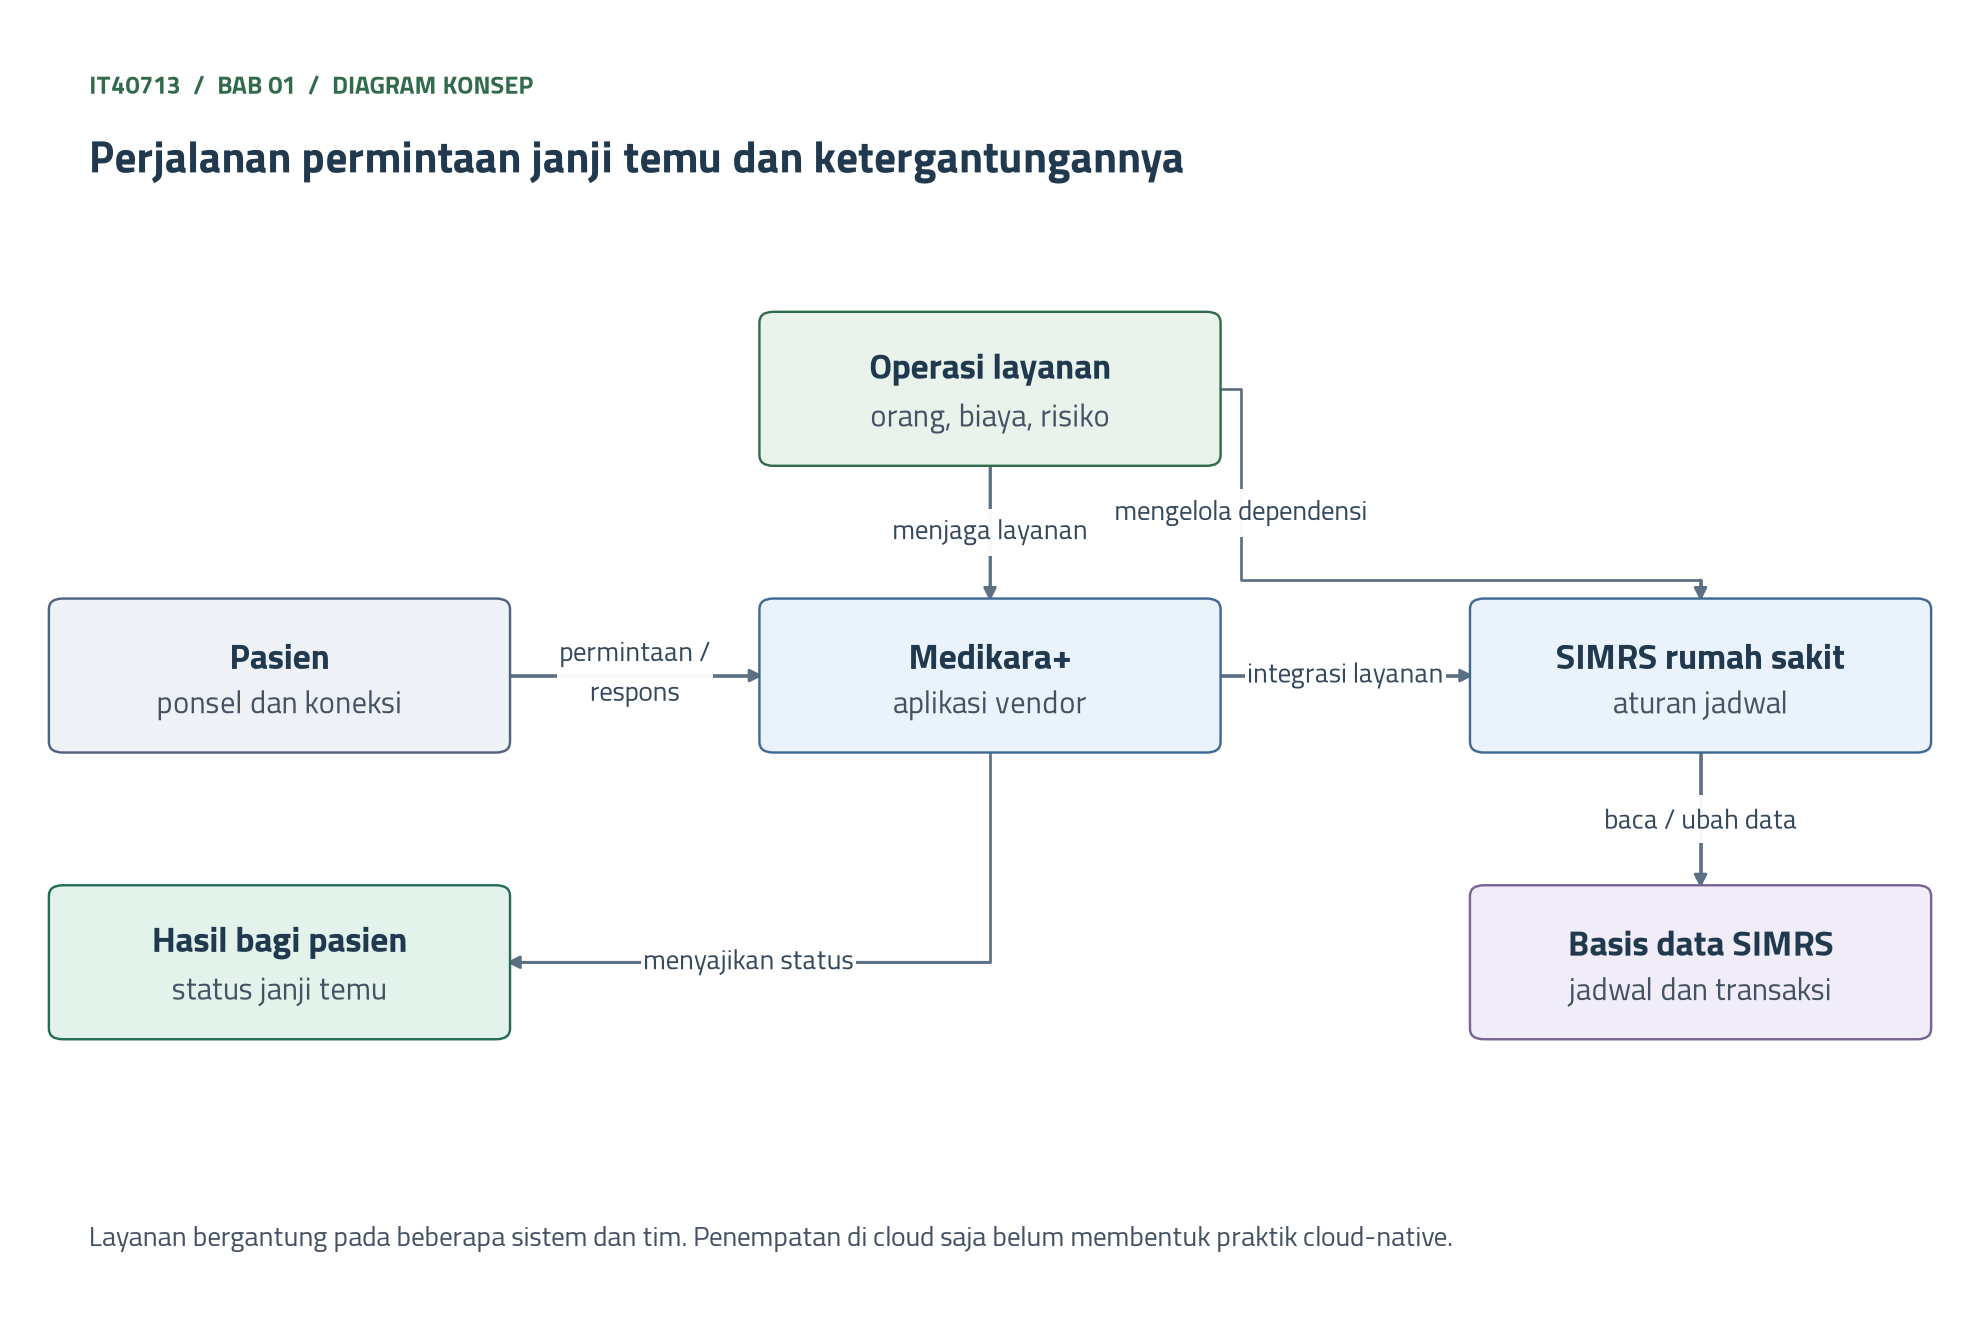
\includegraphics[width=\textwidth]{../figures/ch01-diagram-konsep.png}
  \caption{Perjalanan permintaan janji temu dan ketergantungannya}
  \label{fig:ch01-bahasa-bersama}
\end{figure}

\subsection{Aplikasi, Server, dan Basis Data}

Aplikasi adalah program yang dipakai orang untuk menyelesaikan pekerjaan, misalnya
mendaftarkan pasien, membuat janji temu, atau mencatat tagihan. Server adalah komputer
yang menjalankan aplikasi bagi banyak pengguna sekaligus. Server menyala terus-menerus
dan biasanya ditaruh di ruangan khusus. Basis data adalah tempat data disimpan secara
teratur agar bisa dicari, diubah, dan dijaga. Ketiganya bekerja bersama: pengguna
menyentuh tampilan aplikasi, aplikasi mengerjakan perintah di server, dan hasilnya
dicatat di basis data.

Analoginya adalah restoran. Ruang makan dan daftar menu adalah tampilan aplikasi, tempat
pelanggan memesan. Dapur dan para koki adalah server yang mengerjakan pesanan. Gudang
bahan dan buku catatan stok adalah basis data. Pelanggan tidak masuk ke dapur dan tidak
membuka gudang. Pelanggan cukup memesan, lalu menerima hasilnya.

Dua contoh di Medikara Health:
\begin{enumerate}
  \item SIMRS rumah sakit Jakarta dipakai sekitar 900 pengguna setiap hari, yaitu
        dokter, perawat, petugas pendaftaran, dan kasir. Aplikasi itu berjalan di server
        di ruang server rumah sakit, dan riwayat kunjungan tersimpan di basis data SIMRS.
  \item ERP keuangan adalah satu aplikasi untuk 36 fasilitas: 5 rumah sakit, 18 klinik,
        1 laboratorium, dan 12 apotek. Karena terpusat, laporan keuangan bulanan disusun
        dari satu basis data, tidak perlu menggabungkan 36 berkas terpisah.
\end{enumerate}

\subsection{Jaringan dan Pusat Data}

Jaringan adalah jalur yang menghubungkan perangkat agar dapat bertukar data. Internet
adalah jaringan publik yang dipakai bersama oleh semua orang, sedangkan jaringan
internal adalah jaringan milik organisasi yang menghubungkan kantor dan fasilitasnya.
Pusat data adalah gedung atau ruangan khusus tempat server dijalankan, lengkap dengan
listrik cadangan, pendingin, dan pengamanan fisik. Keandalan keduanya menentukan apakah
aplikasi bisa dipakai saat dibutuhkan.

Analoginya adalah jalan raya dan gudang logistik. Jaringan adalah jalan yang dilalui
kurir. Bila jalan terputus, barang terlambat walaupun gudangnya penuh. Pusat data
adalah gudang besar berpendingin, dijaga satpam, dan punya genset sendiri. Gudang yang
bagus tidak menolong bila jalan menuju gudang itu putus.

Dua contoh di Medikara Health:
\begin{enumerate}
  \item Misalkan jaringan internal dari satu klinik pratama di Bogor ke SIMRS rumah
        sakit Bogor terputus 2 jam. Pendaftaran dicatat di kertas lalu diketik ulang,
        sekitar 60 pendaftaran tercatat dua kali, dan petugas lembur untuk menyamakannya.
  \item Ruang server rumah sakit Depok hanya punya satu unit pendingin. Ketika unit itu
        rusak pada siang hari, server harus dimatikan dan SIMRS berhenti sekitar 90
        menit.
\end{enumerate}

\subsection{Cloud sebagai Layanan Komputasi yang Disewa}

NIST mendefinisikan \textit{cloud computing} sebagai model yang memberi akses lewat
jaringan, kapan pun dibutuhkan, ke kumpulan sumber daya komputasi bersama, seperti
jaringan, server, penyimpanan, aplikasi, dan layanan. Sumber daya itu dapat disediakan
dan dilepas dengan cepat, dengan upaya pengelolaan yang kecil \cite{nist800-145}.
Definisi yang sama menyebut lima karakteristik esensial: swalayan sesuai permintaan,
akses jaringan yang luas, penggabungan sumber daya, elastisitas yang cepat, dan layanan
yang terukur. Bab 2 membahasnya lebih rinci. Bagi manajemen, intinya sederhana:
\textit{cloud} adalah layanan komputasi yang disewa sesuai pemakaian, kapasitasnya
dapat ditambah atau dikurangi dengan cepat, tetapi tanggung jawab atas data dan cara
pemakaiannya tidak ikut berpindah.

Analoginya adalah menyewa mobil dibandingkan membeli mobil sendiri. Penyewa tidak perlu
membayar harga mobil di muka, tidak mengurus servis, dan dapat memilih mobil besar
hanya pada hari libur. Namun, bila mobil dipakai setiap hari untuk jarak jauh, membeli
sendiri bisa lebih murah. Penyewa juga tetap bertanggung jawab atas cara mengemudi dan
barang yang dibawanya.

Dua contoh di Medikara Health:
\begin{enumerate}
  \item Misalkan pemakaian Medikara+ pada Senin pagi mencapai 4 kali rata-rata harian.
        Dengan server sendiri, kapasitas harus dibeli untuk puncak itu, padahal
        kapasitas tersebut menganggur hampir sepanjang pekan. Di \textit{cloud},
        kapasitas tambahan disewa hanya selama beberapa jam puncak.
  \item Laporan konsolidasi keuangan dihitung sekali sebulan selama sekitar 6 jam.
        Server sewaan untuk pekerjaan itu cukup dinyalakan 6 dari 720 jam dalam sebulan.
\end{enumerate}

Tabel \ref{tab:ch01-istilah} merangkum keenam istilah beserta analoginya. Tabel ini
dapat dipakai sebagai kamus kecil saat tim berdiskusi.

\begin{table}[!htb]
  \centering
  \small
  \caption{Enam istilah dasar sistem informasi dengan bahasa sehari-hari}
  \label{tab:ch01-istilah}
  \begin{tabularx}{\textwidth}{P{2cm}LP{3.6cm}}
    \hline
    \textbf{Istilah} & \textbf{Arti sederhana} & \textbf{Analogi} \\
    \hline
    Aplikasi & Program untuk menyelesaikan pekerjaan & Ruang makan dan menu \\
    \hline
    Server & Komputer yang menjalankan aplikasi bagi banyak pengguna & Dapur dan koki \\
    \hline
    Basis data & Tempat data disimpan teratur & Gudang bahan dan buku stok \\
    \hline
    Jaringan & Jalur yang menghubungkan perangkat & Jalan raya \\
    \hline
    Pusat data & Ruang server dengan listrik cadangan dan pendingin & Gudang berpendingin
      dengan genset \\
    \hline
    \textit{Cloud} & Layanan komputasi yang disewa sesuai pemakaian & Menyewa mobil \\
    \hline
  \end{tabularx}
\end{table}

\subsection{Perjalanan Satu Permintaan}

Keenam istilah tadi bertemu dalam satu peristiwa sederhana: pasien memesan janji temu
lewat ponsel. Gambar \ref{fig:ch01-perjalanan-permintaan} memperlihatkan perjalanan
permintaan itu dalam enam langkah. Permintaan berangkat dari aplikasi di ponsel,
menempuh jaringan, diolah server aplikasi milik vendor, diteruskan lewat penghubung
integrasi ke SIMRS rumah sakit, lalu dicatat di basis data. Jawabannya kembali ke ponsel
pasien.

\begin{figure}[!htb]
  \centering
  % Perjalanan satu permintaan janji temu dari aplikasi Medikara+ sampai ke basis
% data SIMRS rumah sakit, lalu jawabannya kembali ke ponsel pasien.
\begin{tikzpicture}[
  font=\scriptsize,
  kotak/.style={draw, rounded corners, align=center, minimum height=1.05cm,
                text width=2.5cm},
  nomor/.style={circle, draw, fill=white, inner sep=1pt, font=\tiny\bfseries},
  panah/.style={-{Stealth[length=2mm]}, thick}
]
  \node[kotak, fill=blue!8] (ponsel) at (0,0)
    {\textbf{Ponsel pasien}\\{\tiny\mdseries aplikasi Medikara+}};
  \node[kotak, fill=blue!8] (jaringan) at (3.7,0)
    {\textbf{Jaringan}\\{\tiny\mdseries internet dan\\operator seluler}};
  \node[kotak, fill=blue!8] (aplikasi) at (7.4,0)
    {\textbf{Server aplikasi}\\{\tiny\mdseries Medikara+ milik vendor}};
  \node[kotak, fill=orange!12] (integrasi) at (7.4,-2.5)
    {\textbf{Penghubung integrasi}\\{\tiny\mdseries \textit{point-to-point}, satu per rumah sakit}};
  \node[kotak, fill=blue!8] (simrs) at (3.7,-2.5)
    {\textbf{SIMRS rumah sakit}\\{\tiny\mdseries server \textit{on-premise}}};
  \node[kotak, fill=green!10] (basisdata) at (0,-2.5)
    {\textbf{Basis data SIMRS}\\{\tiny\mdseries jadwal dokter dan data pasien}};

  \begin{scope}[on background layer]
    \node[draw, dashed, gray, rounded corners, inner sep=6pt,
          fit=(aplikasi) (integrasi)] (vendor) {};
    \node[draw, dashed, gray, rounded corners, inner sep=6pt,
          fit=(simrs) (basisdata)] (rumahsakit) {};
  \end{scope}
  \node[font=\tiny, gray, anchor=south east] at (vendor.north east) {pusat data vendor};
  \node[font=\tiny, gray, anchor=north west] at (rumahsakit.south west)
    {pusat data rumah sakit};

  \draw[panah] (ponsel) -- node[nomor, above=2pt] {1} (jaringan);
  \draw[panah] (jaringan) -- node[nomor, above=2pt] {2} (aplikasi);
  \draw[panah] (aplikasi) -- node[nomor, right=2pt] {3} (integrasi);
  \draw[panah] (integrasi) -- node[nomor, above=2pt] {4} (simrs);
  \draw[panah] (simrs) -- node[nomor, above=2pt] {5} (basisdata);
  \draw[panah, dashed, praditagreen] (basisdata.north) -- node[nomor, left=2pt] {6}
    node[pos=0.5, right, font=\tiny, text=praditagreen, align=left]
      {jawaban: slot\\terkonfirmasi} (ponsel.south);
\end{tikzpicture}

  \caption{Perjalanan satu permintaan janji temu dari Medikara+ sampai ke basis data
           SIMRS, lalu kembali ke ponsel pasien}
  \label{fig:ch01-perjalanan-permintaan}
\end{figure}

\begin{kasus}[title={Kasus Medikara Health: Janji Temu dari Medikara+}]
  Seorang pasien membuka Medikara+ pada Senin pukul 07.10 dan memilih dokter penyakit
  dalam di rumah sakit Bandung. Langkah 1 dan 2 membawa permintaan lewat jaringan seluler
  dan internet ke server aplikasi Medikara+ di pusat data vendor. Server itu tidak
  menyimpan jadwal dokter, sehingga pada langkah 3 permintaan diteruskan ke penghubung
  integrasi khusus rumah sakit Bandung. Pada langkah 4 dan 5, penghubung menerjemahkan
  permintaan ke format SIMRS Bandung, lalu SIMRS memeriksa slot di basis datanya.
  Langkah 6 mengirim jawaban "slot terkonfirmasi" kembali ke ponsel.

  Misalkan pasien menunggu 25 detik lalu mendapat pesan gagal. Pasien hanya tahu
  "aplikasinya lambat". Sumber masalahnya bisa ada di enam titik: sinyal ponsel,
  jaringan, server vendor yang penuh, penghubung Bandung yang belum diperbarui setelah
  SIMRS Bandung naik versi, SIMRS yang sedang menjalankan proses cadangan, atau basis
  data yang lambat. Karena lima rumah sakit memakai lima versi SIMRS, Medikara+
  membutuhkan lima penghubung berbeda, dan setiap perubahan di satu SIMRS berpotensi
  merusak satu penghubung.

  Pelajaran dari kasus ini: keluhan pengguna adalah gejala, bukan diagnosis. Daftar
  pemicu modernisasi pada Aktivitas bab ini harus memisahkan keluhan yang dirasakan dari
  sistem yang diduga menjadi penyebabnya.
\end{kasus}

\section{Bahasa Bersama untuk Mahasiswa Teknis}

Mahasiswa berlatar TI biasanya fasih menyebut komponen, tetapi sering kesulitan
menjelaskan mengapa sebuah perubahan layak dibiayai. Direksi jarang bertanya tentang
jenis basis data. Direksi bertanya apakah perubahan itu menambah pendapatan, mengurangi
biaya, menurunkan risiko, atau memperbaiki layanan pasien, dan berapa lama modalnya
kembali. Bagian ini membahas empat hal yang membentuk bahasa manajemen: nilai bisnis,
struktur biaya, risiko dan kepatuhan, serta cara menulis rekomendasi.

\subsection{Nilai Bisnis dan Cara Manajemen Menilainya}

Nilai bisnis adalah manfaat yang dapat diukur bagi organisasi. Bentuknya antara lain
pendapatan yang bertambah, biaya yang turun, risiko yang mengecil, pelanggan yang lebih
puas, dan kepatuhan yang terjaga. Manajemen menilainya lewat indikator kinerja utama,
atau Key Performance Indicator (KPI), misalnya waktu tunggu pendaftaran, jumlah
kunjungan, dan biaya per kunjungan. Usulan teknologi yang tidak bisa dikaitkan dengan
salah satu KPI biasanya kalah bersaing dengan usulan lain di rapat anggaran.

Analoginya adalah pemilik warung kopi yang ditawari mesin kopi baru. Pemilik itu tidak
terkesan oleh angka tekanan uap atau suhu ketel. Pertanyaannya hanya dua: berapa cangkir
tambahan yang terjual per hari, dan berapa bulan modalnya kembali. Penjual yang menjawab
dua pertanyaan itu dengan angka lebih mungkin berhasil daripada penjual yang membacakan
brosur spesifikasi.

Dua contoh di Medikara Health:
\begin{enumerate}
  \item Usulan "memperbarui server SIMRS rumah sakit Bekasi" sulit dinilai direksi.
        Usulan yang sama dapat ditulis ulang menjadi "memangkas waktu tunggu pendaftaran
        Senin pagi dari rata-rata 70 menit menjadi 30 menit". Kalimat kedua menyebut KPI
        yang dipantau direksi setiap bulan.
  \item Misalkan pada jam sibuk telekonsultasi Medikara+ melayani sekitar 60 sesi per
        jam dengan tarif rata-rata Rp150.000. Setiap jam aplikasi tidak bisa dipakai pada
        jam sibuk berarti pendapatan sekitar 60 × Rp150.000 = Rp9 juta yang hilang,
        belum termasuk pasien yang kecewa dan beralih ke penyedia lain.
\end{enumerate}

Tabel \ref{tab:ch01-terjemahan} memperlihatkan cara menerjemahkan temuan teknis ke dalam
bahasa dampak. Kolom tengah berisi pertanyaan yang hampir pasti diajukan direksi saat
membaca kolom pertama.

\begin{table}[!htb]
  \centering
  \footnotesize
  \caption{Menerjemahkan temuan teknis ke dalam bahasa dampak bagi direksi}
  \label{tab:ch01-terjemahan}
  \begin{tabularx}{\textwidth}{LP{2.5cm}L}
    \hline
    \textbf{Bahasa teknis} & \textbf{Pertanyaan direksi} & \textbf{Bahasa dampak} \\
    \hline
    Server SIMRS Bekasi sering kehabisan memori & Apa akibatnya bagi pasien? &
      Pendaftaran berhenti rata-rata 3 kali sebulan, masing-masing sekitar 40 menit \\
    \hline
    Integrasi ke lima SIMRS masih \textit{point-to-point} & Berapa biayanya? & Setiap
      mitra baru membutuhkan lima penghubung, sehingga satu kerja sama baru tertunda
      sekitar 4 bulan \\
    \hline
    Akun vendor tidak punya masa berlaku & Seberapa besar risikonya? & Insiden 2025
      terjadi lewat jalur yang sama dan wajib dilaporkan dalam 3 kali 24 jam \\
    \hline
    Laporan manajemen disusun dari \textit{spreadsheet} & Apa yang hilang? & Laporan
      bulanan baru siap pada tanggal 12, sehingga keputusan selalu terlambat dua pekan \\
    \hline
  \end{tabularx}
\end{table}

\subsection{Struktur Biaya dan Siklus Anggaran}

Biaya TI dicatat dalam dua kelompok besar. Belanja modal, atau Capital Expenditure
(CapEx), adalah pembelian aset yang dibayar di muka dan disusutkan selama beberapa
tahun, misalnya server dan perangkat jaringan. Belanja operasional, atau Operational
Expenditure (OpEx), adalah pengeluaran rutin yang dibayar selama layanan dipakai,
misalnya sewa \textit{cloud}, lisensi bulanan, dan listrik. Pindah ke \textit{cloud}
umumnya menggeser sebagian biaya dari CapEx ke OpEx, dan pergeseran itu mengubah cara
organisasi merencanakan serta mengendalikan anggaran \cite{storment2023}. Biaya yang
dibandingkan juga tidak cukup harga beli. Biaya total kepemilikan, atau Total Cost of
Ownership (TCO), mencakup listrik, pendingin, ruang, lisensi, staf yang merawat, dan
penggantian perangkat. Bab 3 membahas TCO dan pengelolaan biaya \textit{cloud} secara
rinci.

Analoginya adalah mesin fotokopi kantor. Kantor dapat membeli mesin seharga Rp60 juta,
membayarnya di muka, dan merawatnya sendiri. Kapasitasnya tetap, entah dipakai 100
lembar atau 10.000 lembar sebulan. Kantor juga dapat menyewa mesin dengan tarif per
lembar. Tagihannya berubah setiap bulan mengikuti pemakaian, dan bagian keuangan harus
siap dengan tagihan yang naik saat musim laporan.

Siklus anggaran ikut menentukan. Di banyak organisasi, anggaran tahun berikutnya disusun
dan disetujui beberapa bulan sebelum tahun berjalan. Anggaran CapEx cocok dengan siklus
itu karena angkanya tetap. Tagihan \textit{cloud} yang naik turun setiap bulan perlu
kebiasaan baru: perkiraan pemakaian, batas pengeluaran, label biaya per layanan, dan
peninjauan tagihan secara rutin.

Dua contoh di Medikara Health:
\begin{enumerate}
  \item Misalkan penggantian 6 server SIMRS rumah sakit Bandung ditawarkan seharga Rp1,8
        miliar. Dengan masa susut 5 tahun, beban penyusutannya Rp360 juta per tahun,
        belum termasuk listrik, pendingin, dan staf. Penawaran \textit{cloud} untuk beban
        yang sama misalnya Rp32 juta per bulan, atau Rp384 juta per tahun. Angka mentah
        ini belum cukup untuk memutuskan, karena kedua sisi belum dihitung sebagai TCO.
  \item Tagihan \textit{cloud} Medikara+ bulan Januari Rp28 juta, lalu bulan Februari
        Rp41 juta karena kampanye pendaftaran vaksinasi. Bagian keuangan bertanya
        mengapa tagihan naik 46 persen. Tanpa label biaya per layanan, tim TI tidak
        dapat menjawab dengan cepat.
\end{enumerate}

\subsection{Risiko dan Kepatuhan sebagai Batasan Desain}

Risiko adalah kemungkinan terjadinya peristiwa yang merugikan, dikalikan dengan
dampaknya. Kepatuhan adalah keadaan ketika organisasi memenuhi aturan yang wajib
diikuti, baik dari undang-undang, regulator, maupun kontrak. Bagi perancang sistem,
keduanya bukan lampiran yang ditambahkan menjelang proyek selesai, melainkan batasan
desain sejak hari pertama, seperti beban maksimum yang harus ditahan sebuah jembatan.

Di sektor kesehatan Indonesia, dua aturan langsung membentuk batasan itu. Undang-Undang
(UU) Nomor 27 Tahun 2022 tentang Pelindungan Data Pribadi (PDP) menggolongkan data dan
informasi kesehatan sebagai data pribadi yang bersifat spesifik. UU yang sama mewajibkan
pengendali data menyampaikan pemberitahuan tertulis paling lambat 3 kali 24 jam bila
terjadi kegagalan pelindungan data pribadi, dan mengatur sanksi administratif berupa
denda paling tinggi 2 persen dari pendapatan tahunan \cite{uu27-2022-pdp}. Peraturan
Menteri Kesehatan (Permenkes) Nomor 24 Tahun 2022 tentang Rekam Medis mewajibkan
fasilitas pelayanan kesehatan menyelenggarakan rekam medis elektronik paling lambat 31
Desember 2023. Permenkes yang sama mengizinkan rekam medis elektronik disimpan di server,
di \textit{cloud computing} yang tersertifikasi, atau di media digital lain
\cite{permenkes24-2022}. Aturan tentang lokasi pengelolaan data dibahas pada Bab 2.

Analoginya adalah aturan keselamatan gedung. Tangga darurat, pintu tahan api, dan jalur
evakuasi ditentukan saat denah digambar. Menambahkan tangga darurat setelah gedung
berdiri jauh lebih mahal, kadang mustahil tanpa membongkar dinding. Kontrol akses,
catatan jejak akses, dan pemisahan data sensitif bekerja dengan cara yang sama.

\begin{kasus}[title={Kasus Medikara Health: Insiden Vendor dan Temuan Audit}]
  Pada 2025, data sebagian pasien Medikara+ terbuka lewat akun milik vendor aplikasi.
  Akun itu dibuat untuk keperluan uji, punya hak akses luas, dan masih aktif setelah
  proyeknya selesai. Skala insidennya kecil, tetapi Medikara Health tetap harus
  menelusuri data mana yang terbuka dan memberi tahu pasien yang terdampak. Tak lama
  kemudian, audit internal menemukan kontrol akses yang lemah di beberapa SIMRS:
  akun karyawan yang sudah keluar masih aktif, dan satu akun dipakai bersama oleh
  beberapa petugas. Kedua peristiwa itu kini menjadi batasan desain bagi setiap
  rancangan baru:
  \begin{enumerate}
    \item Setiap akun, termasuk akun vendor, hanya mendapat hak akses yang dibutuhkan
          dan punya masa berlaku.
    \item Setiap akses ke data pasien tercatat dan dapat diaudit.
    \item Organisasi harus dapat mengetahui data siapa yang terdampak dalam waktu kurang
          dari 3 kali 24 jam. Syarat ini menuntut katalog data yang jelas.
  \end{enumerate}
  Batasan ketiga menunjukkan bahwa regulasi ikut menentukan arsitektur. Tanpa mengetahui
  letak data pasien, kewajiban pelaporan tidak mungkin dipenuhi tepat waktu.
\end{kasus}

\subsection{Menulis Rekomendasi untuk Direksi}

Rekomendasi untuk direksi ditulis ringkas, paling panjang satu halaman, dengan jawaban
di bagian depan. Prinsip ini dikenal sebagai prinsip piramida: kesimpulan disampaikan
lebih dahulu, lalu didukung beberapa alasan, dan setiap alasan didukung data
\cite{c01-minto2009}. Isi rekomendasi berbasis dampak, menyebut pilihan lain yang
dipertimbangkan, menyatakan \textit{trade-off} secara jujur, dan meminta keputusan yang
jelas. Rekomendasi yang hanya menjelaskan teknologi tanpa meminta keputusan biasanya
berakhir dengan "akan dipelajari lebih lanjut".

Analoginya adalah dokter yang menjelaskan pilihan tindakan kepada keluarga pasien.
Dokter menyampaikan diagnosis singkat, dua atau tiga pilihan tindakan, risiko
masing-masing, lalu sarannya. Keputusan akhir ada di tangan keluarga. Dokter tidak
membacakan buku ajar farmakologi, dan keluarga tidak dibiarkan menebak pilihan mana
yang disarankan.

Dua contoh kalimat pembuka:
\begin{enumerate}
  \item Lemah: "Disarankan migrasi SIMRS ke \textit{microservices} di Kubernetes agar
        lebih \textit{scalable}." Masalah, dampak, biaya, dan keputusannya tidak ada.
  \item Kuat: "Direksi diminta menyetujui uji coba pendaftaran daring terpadu di Bekasi
        selama 3 bulan, Rp420 juta, dengan sasaran waktu tunggu Senin pagi turun dari
        70 menjadi 30 menit." Susunan lengkapnya ada pada Tabel
        \ref{tab:ch01-rekomendasi}.
\end{enumerate}

\begin{table}[!htb]
  \centering
  \footnotesize
  \caption{Susunan rekomendasi satu halaman untuk direksi beserta contoh isinya}
  \label{tab:ch01-rekomendasi}
  \begin{tabularx}{\textwidth}{P{2.6cm}L}
    \hline
    \textbf{Bagian} & \textbf{Contoh isi untuk Medikara Health} \\
    \hline
    Keputusan yang diminta & Menyetujui uji coba pendaftaran daring terpadu di rumah
      sakit Bekasi selama 3 bulan, biaya Rp420 juta \\
    \hline
    Masalah dan dampak & Waktu tunggu Senin pagi rata-rata 70 menit, sebagian pasien
      pulang sebelum dilayani \\
    \hline
    Pilihan yang dipertimbangkan & (a) Menambah petugas loket, (b) uji coba pendaftaran
      daring terpadu, (c) mengganti seluruh SIMRS \\
    \hline
    Rekomendasi dan alasan & Pilihan (b): menyentuh penyebab utama, biaya terbatas,
      hasilnya terukur dalam 3 bulan \\
    \hline
    \textit{Trade-off} dan risiko & Lebih lambat daripada mengganti seluruh SIMRS dan
      belum menyelesaikan perbedaan versi, tetapi risikonya jauh lebih kecil \\
    \hline
    Langkah berikutnya & Bila sasaran tercapai, perluasan ke rumah sakit Depok dan Bogor
      diusulkan pada anggaran berikutnya \\
    \hline
  \end{tabularx}
\end{table}

\section{Kualitas Sistem dan Trade-off}

Kualitas sistem adalah sifat yang menentukan seberapa baik sistem melayani, di luar
daftar fiturnya. Dua aplikasi janji temu bisa punya fitur yang sama persis, tetapi yang
satu selalu bisa dipakai pada Senin pagi, sedangkan yang lain sering gagal. Mata kuliah
ini memakai lima kualitas utama: ketersediaan, skalabilitas, keamanan, biaya, dan
kecepatan perubahan. Tabel \ref{tab:ch01-kualitas} menjelaskan masing-masing beserta
contoh ukurannya.

\begin{table}[!htb]
  \centering
  \footnotesize
  \caption{Lima kualitas sistem yang dipakai sepanjang mata kuliah ini}
  \label{tab:ch01-kualitas}
  \begin{tabularx}{\textwidth}{P{1.9cm}LLL}
    \hline
    \textbf{Kualitas} & \textbf{Pertanyaan yang dijawab} & \textbf{Contoh ukuran} &
      \textbf{Contoh di Medikara Health} \\
    \hline
    Ketersediaan & Bisakah sistem dipakai saat dibutuhkan? & Persentase waktu sistem
      dapat dipakai, misalnya 99,9 persen & SIMRS instalasi gawat darurat harus hidup
      24 jam \\
    \hline
    Skalabilitas & Sanggupkah sistem melayani beban yang bertambah? & Jumlah permintaan
      per menit yang masih dilayani dengan cepat & Lonjakan janji temu pada Senin
      pagi \\
    \hline
    Keamanan & Terlindungkah data dan akses? & Jumlah akun tanpa masa berlaku, waktu
      menutup celah & Akun vendor dan akun karyawan yang sudah keluar \\
    \hline
    Biaya & Berapa yang dibayar untuk hasil itu? & Biaya infrastruktur per kunjungan
      pasien & Tagihan \textit{cloud} Medikara+ per bulan \\
    \hline
    Kecepatan perubahan & Seberapa cepat perubahan sampai ke pengguna? & Waktu dari
      permintaan perubahan sampai rilis & Fitur baru Medikara+ yang menunggu jadwal
      rilis vendor \\
    \hline
  \end{tabularx}
\end{table}

Dua hal pada kualitas sistem sering tertukar, yaitu ketersediaan dan skalabilitas.
Pembagiannya begini. Ketersediaan menyangkut apakah sistem hidup dan bisa dipakai.
Skalabilitas menyangkut apakah sistem tetap layak dipakai ketika penggunanya bertambah.
Sebuah sistem bisa selalu hidup tetapi lambat sekali pada jam ramai, artinya tersedia
tetapi tidak skalabel. Sebaliknya, sistem yang mampu melayani lonjakan besar bisa tetap
mati total ketika satu-satunya pusat datanya padam.

\subsection{Mengapa Kualitas Saling Tarik-Menarik}

Kelima kualitas tidak dapat dimaksimalkan sekaligus, karena uang, waktu, dan perhatian
tim terbatas. Menaikkan satu kualitas hampir selalu membebani kualitas lain. Gambar
\ref{fig:ch01-tarik-menarik} memperlihatkan lima pasangan yang paling sering
bertentangan. Richards dan Ford merumuskannya sebagai hukum pertama arsitektur perangkat
lunak: setiap keputusan arsitektur adalah \textit{trade-off}. Hukum kedua mereka
menyatakan bahwa alasan sebuah keputusan lebih penting daripada cara melaksanakannya
\cite{richards2025}.

\begin{figure}[!htb]
  \centering
  % Lima kualitas sistem yang saling tarik-menarik. Setiap sisi segi lima
% menandai satu pasangan yang sering bertentangan, dengan contoh singkatnya.
\begin{tikzpicture}[
  font=\scriptsize,
  kualitas/.style={draw, rounded corners, align=center, minimum height=0.85cm,
                   text width=2.1cm, fill=blue!8, font=\scriptsize\bfseries},
  tarik/.style={{Stealth[length=1.8mm]}-{Stealth[length=1.8mm]}, thick, red!60!black,
                dashed},
  catatan/.style={font=\tiny, gray!40!black, align=center}
]
  \node[kualitas] (sedia) at (90:3.1) {Ketersediaan};
  \node[kualitas] (biaya) at (18:3.1) {Biaya};
  \node[kualitas] (skala) at (-54:3.1) {Skalabilitas};
  \node[kualitas] (aman) at (-126:3.1) {Keamanan};
  \node[kualitas] (ubah) at (162:3.1) {Kecepatan\\perubahan};

  \node[draw, rounded corners, align=center, fill=praditagreen!15, text width=2.9cm,
        minimum height=1.1cm, font=\scriptsize] at (0,0)
    {\textbf{Keputusan arsitektur}\\[2pt]
     {\tiny\mdseries memilih titik seimbang\\dan menuliskan alasannya}};

  \draw[tarik] (sedia) -- node[catatan, above right=-1pt] {cadangan di dua lokasi\\menambah biaya} (biaya);
  \draw[tarik] (biaya) -- node[catatan, right=2pt] {kapasitas cadangan\\tetap dibayar} (skala);
  \draw[tarik] (skala) -- node[catatan, below=0.55cm] {lebih banyak komponen,\\lebih banyak celah} (aman);
  \draw[tarik] (aman) -- node[catatan, left=2pt] {pemeriksaan tambahan\\memperlambat rilis} (ubah);
  \draw[tarik] (ubah) -- node[catatan, above left=-1pt] {perubahan sering\\membuka peluang gangguan} (sedia);
\end{tikzpicture}

  \caption{Lima kualitas sistem yang saling tarik-menarik beserta contoh
           pertentangannya}
  \label{fig:ch01-tarik-menarik}
\end{figure}

Analoginya adalah memilih ambulans untuk sebuah klinik. Ambulans dengan peralatan
lengkap lebih mahal dan lebih berat, sehingga lebih lambat di gang sempit. Ambulans
ringan lebih murah dan lincah, tetapi peralatannya terbatas. Tidak ada ambulans yang
sekaligus termurah, terlengkap, dan tercepat. Klinik memilih sesuai wilayah dan pasien
yang dilayaninya, lalu menerima kekurangannya dengan sadar.

Ketersediaan memberi contoh yang paling mudah dihitung. Setiap angka sembilan tambahan
pada target ketersediaan memangkas waktu henti yang diizinkan secara tajam. Tabel
\ref{tab:ch01-ketersediaan} menghitung waktu henti yang masih diizinkan untuk beberapa
target, memakai 8.760 jam per tahun dan 720 jam per bulan. Pengalaman Google dalam
\textit{Site Reliability Engineering} menunjukkan bahwa biaya menambah keandalan naik
jauh lebih cepat daripada manfaatnya, sehingga target perlu disesuaikan dengan
kebutuhan pengguna, bukan dibuat setinggi mungkin \cite{beyer2016}.

\begin{table}[!htb]
  \centering
  \small
  \caption{Waktu henti yang diizinkan untuk beberapa target ketersediaan}
  \label{tab:ch01-ketersediaan}
  \begin{tabularx}{\textwidth}{P{2.2cm}LL}
    \hline
    \textbf{Target} & \textbf{Waktu henti per tahun} &
      \textbf{Waktu henti per bulan (30 hari)} \\
    \hline
    99\% & 87,6 jam (sekitar 3,65 hari) & 7,2 jam \\
    \hline
    99,5\% & 43,8 jam & 3,6 jam \\
    \hline
    99,9\% & 8,76 jam & 43,2 menit \\
    \hline
    99,95\% & 4,38 jam & 21,6 menit \\
    \hline
    99,99\% & 52,6 menit & 4,3 menit \\
    \hline
  \end{tabularx}
\end{table}

Dua contoh \textit{trade-off} di Medikara Health:
\begin{enumerate}
  \item SIMRS untuk instalasi gawat darurat membutuhkan target tinggi, misalnya 99,95
        persen, yang hanya mengizinkan sekitar 4,4 jam henti per tahun. Target itu
        menuntut server cadangan di lokasi lain dan petugas siaga. Laporan konsolidasi
        keuangan bulanan cukup memakai target 99 persen, karena keterlambatan beberapa
        jam tidak membahayakan pasien.
  \item Misalkan setiap rilis Medikara+ wajib melewati pemeriksaan keamanan manual oleh
        tim lain yang hanya bertugas dua kali sebulan. Keamanan membaik, tetapi waktu
        dari permintaan perubahan sampai rilis naik dari 2 pekan menjadi 5 pekan.
        Pilihan lain adalah pemeriksaan otomatis pada setiap perubahan, ditambah
        pemeriksaan manual hanya untuk perubahan yang menyentuh data pasien.
\end{enumerate}

\subsection{Menuliskan Alasan Keputusan}

\textit{Trade-off} yang tidak ditulis akan dilupakan. Dua tahun kemudian, tim baru
melihat keputusan lama dan menilainya keliru, padahal alasannya masuk akal pada waktu
itu. Karena itu, mata kuliah ini membiasakan satu kebiasaan sederhana: setiap keputusan
penting dicatat dalam lima baris, yaitu konteks, keputusan, alasan, \textit{trade-off}
yang diterima, serta tanggal dan pihak yang memutuskan. Bentuk yang lebih baku, yaitu
Architecture Decision Record (ADR), dibahas pada Bab 7. Contoh catatan keputusan untuk
Medikara Health:
\begin{enumerate}
  \item \textbf{Konteks:} telekonsultasi Medikara+ kehilangan sekitar Rp9 juta per jam
        henti pada jam sibuk.
  \item \textbf{Keputusan:} target ketersediaan 99,9 persen, dijalankan di dua lokasi
        dalam satu region.
  \item \textbf{Alasan:} target 99,99 persen menuntut dua region dan biayanya lebih
        besar daripada kerugian yang dicegah.
  \item \textbf{\textit{Trade-off} yang diterima:} bila seluruh region terganggu,
        layanan dapat berhenti beberapa jam.
  \item \textbf{Tanggal dan pemutus:} Januari 2026, direktur operasional bersama kepala
        divisi TI.
\end{enumerate}

\begin{pendalaman}[title={Pendalaman Teknis (opsional): Model Kualitas ISO/IEC 25010}]
  Lima kualitas di bab ini sengaja dibuat sedikit agar mudah dipakai dalam diskusi
  dengan manajemen. Model yang lebih lengkap tersedia di standar ISO/IEC 25010:2023
  tentang model kualitas produk. Edisi 2023 memuat sembilan karakteristik:
  \textit{functional suitability}, \textit{performance efficiency},
  \textit{compatibility}, \textit{interaction capability}, \textit{reliability},
  \textit{security}, \textit{maintainability}, \textit{flexibility}, dan
  \textit{safety}. Setiap karakteristik dirinci lagi menjadi subkarakteristik yang
  dapat dispesifikasikan dan diukur \cite{c01-iso25010}.

  Pemetaan lima kualitas bab ini ke karakteristik terdekat:
  \begin{itemize}
    \item Ketersediaan ke \textit{reliability}, dengan \textit{availability} sebagai
          subkarakteristiknya.
    \item Skalabilitas ke \textit{flexibility} (subkarakteristik \textit{scalability})
          dan \textit{performance efficiency} (subkarakteristik \textit{capacity}).
    \item Keamanan ke \textit{security}; kecepatan perubahan ke
          \textit{maintainability}, walaupun juga ditentukan oleh proses rilis.
    \item Biaya tidak punya padanan sebagai karakteristik produk. Kerangka penyedia
          \textit{cloud} justru menjadikannya pilar tersendiri, misalnya
          \textit{cost optimization} pada AWS Well-Architected Framework
          \cite{awswaf}.
  \end{itemize}
\end{pendalaman}

\section{Arti Cloud-Native bagi Organisasi}

Istilah \textit{cloud-native} sering dipakai seolah-olah sama dengan "sudah di
\textit{cloud}". Dua hal ini sering tertukar. Pembagiannya begini. Aplikasi
\textit{cloud-hosted} adalah aplikasi lama yang dipindahkan apa adanya ke server sewaan
di \textit{cloud}. Cara aplikasi itu dibangun, dirilis, dan ditambah kapasitasnya tidak
berubah. Aplikasi \textit{cloud-native} dirancang, bersama cara kerja timnya, untuk
memanfaatkan sifat \textit{cloud}: kapasitas yang elastis, otomatisasi, dan kemampuan
pulih dari gangguan.

CNCF mendefinisikan praktik \textit{cloud native} sebagai praktik yang memungkinkan
organisasi mengembangkan, membangun, dan men-\textit{deploy} \textit{workload} di
lingkungan komputasi publik, privat, maupun hibrida untuk memenuhi kebutuhannya pada
skala besar, dengan cara yang terprogram dan dapat diulang. Ciri utamanya adalah sistem
yang keterkaitannya longgar dan saling bekerja sama secara aman, tangguh, terkelola,
berkelanjutan, dan dapat diamati \cite{cncf-definition}. Definisi ini dibahas rinci
pada Bab 5. Untuk saat ini, satu hal perlu dicatat: definisi itu berbicara tentang
praktik dan sifat sistem, bukan tentang merek teknologi tertentu.

Analoginya adalah memindahkan warung ke mal. Warung yang pindah ke mal tanpa mengubah
cara kerjanya tetap punya satu kasir dan mencatat stok di buku tulis. Sewanya lebih
mahal, sedangkan antreannya tetap panjang. Toko yang dirancang untuk mal memakai mesin
kasir yang tersambung ke gudang pusat, menambah kasir saat akhir pekan, dan mengisi
ulang stok secara otomatis. Lokasinya sama, hasilnya berbeda karena cara kerjanya ikut
berubah.

Dua contoh di Medikara Health:
\begin{enumerate}
  \item Misalkan SIMRS rumah sakit Bogor dipindahkan apa adanya ke mesin virtual di
        \textit{cloud}. Ruang server dan pendingin tidak dibutuhkan lagi. Namun, rilis
        tetap dua kali setahun, kapasitas tetap ditambah secara manual, dan satu
        kesalahan masih dapat menghentikan seluruh SIMRS. Ini contoh
        \textit{cloud-hosted}.
  \item Layanan janji temu Medikara+ dirancang ulang sebagai layanan tersendiri.
        Kapasitasnya bertambah otomatis pada Senin pagi, perubahan dirilis setiap pekan
        lewat alur otomatis, dan gangguan pada satu rumah sakit tidak menghentikan
        pemesanan di rumah sakit lain. Ini lebih dekat ke \textit{cloud-native}.
\end{enumerate}

Tabel \ref{tab:ch01-hosted-native} merangkum perbedaannya pada lima aspek.

\begin{table}[!htb]
  \centering
  \small
  \caption{Perbedaan aplikasi \textit{cloud-hosted} dan \textit{cloud-native}}
  \label{tab:ch01-hosted-native}
  \begin{tabularx}{\textwidth}{P{2.4cm}LL}
    \hline
    \textbf{Aspek} & \textbf{\textit{Cloud-hosted}} & \textbf{\textit{Cloud-native}} \\
    \hline
    Bentuk aplikasi & Sama seperti di pusat data lama & Dirancang ulang menjadi bagian
      yang longgar keterkaitannya \\
    \hline
    Menambah kapasitas & Manual, menunggu permintaan & Otomatis mengikuti beban \\
    \hline
    Cara rilis & Jarang, terjadwal, berisiko besar & Sering, kecil, lewat alur
      otomatis \\
    \hline
    Saat terjadi gangguan & Satu kesalahan dapat menghentikan semuanya & Gangguan
      dibatasi pada satu bagian \\
    \hline
    Yang ikut berubah & Lokasi server & Lokasi, rancangan aplikasi, dan cara kerja
      tim \\
    \hline
  \end{tabularx}
\end{table}

\subsection{Mitos yang Sering Menyertai Cloud-Native}

Pertanyaan kemudian muncul: bila \textit{cloud-native} punya banyak keunggulan, mengapa
tidak semua organisasi langsung menerapkannya? Jawabannya, keunggulan itu datang
bersama biaya dan kerumitan baru. Sejumlah mitos membuat keduanya terlupa. Tabel
\ref{tab:ch01-mitos} merangkum lima mitos yang paling sering muncul di rapat
manajemen.

\begin{table}[!htb]
  \centering
  \footnotesize
  \caption{Lima mitos tentang \textit{cloud} dan \textit{cloud-native} beserta
           kenyataannya}
  \label{tab:ch01-mitos}
  \begin{tabularx}{\textwidth}{P{3.1cm}L}
    \hline
    \textbf{Mitos} & \textbf{Kenyataan} \\
    \hline
    \textit{Cloud} selalu lebih murah & Bergantung pada pola pemakaian dan disiplin
      pengelolaan. Dalam survei Flexera 2026, responden memperkirakan sekitar 29 persen
      belanja \textit{cloud} mereka terbuang \cite{flexera2026}. \\
    \hline
    \textit{Microservices} selalu lebih baik & Memecah aplikasi menambah kerumitan
      operasi. Segment pernah menggabungkan kembali ratusan layanan kecilnya menjadi
      satu layanan karena beban perawatannya terlalu berat \cite{noonan2018}. \\
    \hline
    Pindah ke \textit{cloud} otomatis lebih aman & Penyedia mengamankan
      infrastrukturnya, tetapi akun, hak akses, dan konfigurasi tetap tanggung jawab
      pelanggan (Bab 2). \\
    \hline
    \textit{Cloud-native} berarti harus memakai Kubernetes & Definisi CNCF menekankan
      praktik dan sifat sistem, bukan alat tertentu \cite{cncf-definition}. \\
    \hline
    Sekali pindah, urusan selesai & Modernisasi berlangsung bertahap selama
      bertahun-tahun dan dikelola sebagai peta jalan (Bab 14). \\
    \hline
  \end{tabularx}
\end{table}

\subsection{Perjalanan Mata Kuliah}

Setiap mitos di atas dijawab oleh satu atau beberapa pertemuan. Gambar
\ref{fig:ch01-perjalanan-mk} memperlihatkan perjalanan mata kuliah dalam empat Bagian.
Bagian I menjawab mengapa organisasi perlu berubah, batasan apa yang mengikat, dan
berapa biayanya. Bagian II membaca kondisi saat ini. Bagian III merancang arsitektur
target. Bagian IV menyusun cara sistem dijalankan, dipulihkan, dan dimodernisasi secara
bertahap. Bab ini adalah titik awal Bagian I.

\begin{figure}[!htb]
  \centering
  % Perjalanan mata kuliah IT40713 dalam empat Bagian, dari strategi sampai peta
% jalan, beserta pertanyaan utama yang dijawab tiap Bagian.
\begin{tikzpicture}[
  font=\scriptsize,
  bagian/.style={draw, rounded corners, align=center, minimum height=1.15cm,
                 text width=2.4cm, font=\scriptsize\bfseries},
  tanya/.style={align=center, text width=2.5cm, font=\tiny, gray!30!black},
  panah/.style={-{Stealth[length=2mm]}, thick}
]
  \node[bagian, fill=orange!12] (b1) at (0,0)
    {Bagian I\\Fondasi dan Strategi\\{\tiny\mdseries Pertemuan 1 sampai 3}};
  \node[bagian, fill=blue!8] (b2) at (3.1,0)
    {Bagian II\\Kondisi Saat Ini\\{\tiny\mdseries Pertemuan 4 sampai 7}};
  \node[bagian, fill=blue!8] (b3) at (6.2,0)
    {Bagian III\\Arsitektur Target\\{\tiny\mdseries Pertemuan 8 sampai 11}};
  \node[bagian, fill=green!10] (b4) at (9.3,0)
    {Bagian IV\\Operasi dan Peta Jalan\\{\tiny\mdseries Pertemuan 12 sampai 14}};

  \draw[panah] (b1) -- (b2);
  \draw[panah] (b2) -- (b3);
  \draw[panah] (b3) -- (b4);

  \node[tanya, below=4pt of b1] {Mengapa berubah?\\Apa batasannya?\\Berapa biayanya?};
  \node[tanya, below=4pt of b2] {Aplikasi mana yang siap?\\Di mana batas\\layanannya?};
  \node[tanya, below=4pt of b3] {Dijalankan di mana?\\Berkomunikasi bagaimana?\\Seberapa andal?};
  \node[tanya, below=4pt of b4] {Bagaimana dipulihkan?\\Urutan modernisasi?\\Siapa yang mengawasi?};

  \node[draw, fill=praditagreen!15, rounded corners, font=\tiny\bfseries,
        inner sep=2pt] (bab1) at ([yshift=10pt]b1.north) {Bab 1: titik awal};
  \node[font=\tiny\bfseries, gray!30!black] at ($(b2.north)!0.5!(b3.north)+(0,0.3)$) {UTS};
  \node[font=\tiny\bfseries, gray!30!black] at ([yshift=10pt]b4.north) {UAS};
\end{tikzpicture}

  \caption{Perjalanan mata kuliah dalam empat Bagian, dari strategi sampai peta jalan
           modernisasi}
  \label{fig:ch01-perjalanan-mk}
\end{figure}

\begin{kasus}[title={Kasus Medikara Health: Pertanyaan dari "Satu Pasien, Satu Rekam Medis"}]
  Strategi "Satu Pasien, Satu Rekam Medis" terdengar sederhana: setiap pasien punya satu
  rekam medis yang dapat dibaca di fasilitas mana pun milik Medikara Health, juga oleh
  mitra yang berhak. Bagi arsitek, strategi itu memunculkan sejumlah pertanyaan:
  \begin{enumerate}
    \item Di mana rekam medis terpadu disimpan, dan aturan apa yang membatasi? (Bab 2)
    \item Berapa biaya infrastruktur per kunjungan pasien? (Bab 3)
    \item Apakah lima SIMRS diseragamkan, diganti, atau dibungkus? (Bab 4 sampai 7, diputuskan di Bab 14)
    \item Bagaimana mitra tersambung tanpa integrasi \textit{point-to-point} baru? (Bab 9)
    \item Bagaimana rekam medis dipulihkan bila satu pusat data padam? (Bab 12)
  \end{enumerate}
  Tidak satu pun pertanyaan itu terjawab dengan "pindahkan semuanya ke \textit{cloud}".
  Setiap jawaban menuntut pilihan beserta \textit{trade-off}-nya, dan pilihan itu
  disusun bertahap sepanjang semester.
\end{kasus}

\section{Aktivitas: Membentuk Tim dan Memetakan Pemicu Modernisasi}

\textbf{Tujuan.} Tim campuran terbentuk, organisasi capstone dipilih, dan masalah TI
yang dirasakan di organisasi itu dirumuskan sebagai pemicu modernisasi. Pemicu
modernisasi adalah masalah nyata yang membuat organisasi perlu mengubah sistemnya,
ditulis lengkap dengan dampak dan sistem yang terlibat. Daftar ini menjadi pijakan
seluruh artefak berikutnya, sehingga mutunya menentukan mutu cetak biru.

\textbf{Pembagian peran.} Tim berisi tiga sampai lima orang, dengan sedikitnya satu
anggota berlatar teknis dan satu anggota berlatar non-teknis. Pada tim tiga orang, satu
anggota boleh memegang dua peran.
\begin{itemize}
  \item \textbf{Koordinator} (anggota mana pun): mengatur jadwal, menyatukan draf, dan
        mewakili tim saat tatap muka Sabtu.
  \item \textbf{Pemimpin wawancara} (anggota non-teknis): memimpin wawancara singkat
        atau penelusuran dokumen tentang masalah layanan.
  \item \textbf{Pemeta sistem} (anggota teknis): memetakan aplikasi, server, basis data,
        dan integrasi yang terlibat dalam setiap masalah.
  \item \textbf{Penjaga izin dan etika} (anggota yang dekat dengan organisasi): mengurus
        izin tertulis dan memeriksa anonimisasi setiap dokumen.
\end{itemize}

\textbf{Langkah kerja.}
\begin{enumerate}
  \item Bentuk tim berisi tiga sampai lima orang dengan latar belakang campuran, lalu
        tetapkan peran.
  \item Pilih organisasi. Bila memakai organisasi nyata, urus izin tertulis dengan
        mengikuti \berkas{sources/chapter01/panduan-izin-dan-anonimisasi.md}. Bila izin
        tidak didapat sampai Pertemuan 2, pakai kasus Medikara Health.
  \item Kumpulkan masalah dari pengguna dan manajemen. Pemimpin wawancara berbicara
        dengan tiga sampai lima orang, misalnya petugas layanan, kepala unit, dan staf
        TI, masing-masing sekitar 20 menit. Catat keluhan apa adanya beserta angka yang
        disebut narasumber. Tim Medikara Health memakai kotak kasus di bab ini sebagai
        pengganti wawancara.
  \item Petakan sistem yang terkait dengan setiap masalah. Pemeta sistem menelusuri
        perjalanan permintaan seperti pada Gambar \ref{fig:ch01-perjalanan-permintaan}
        dan menandai titik yang diduga menjadi penyebab.
  \item Tulis profil organisasi satu halaman memakai
        \berkas{sources/chapter01/templat-profil-organisasi.md}, lalu susun lima sampai
        sepuluh pemicu modernisasi memakai
        \berkas{sources/chapter01/lembar-pemicu-modernisasi.md}. Seluruh anggota
        menyepakati urutan prioritasnya.
\end{enumerate}

\textbf{Luaran dan kaitan dengan capstone.} Tiga dokumen: profil organisasi satu
halaman, daftar lima sampai sepuluh pemicu modernisasi beserta prioritasnya, dan bukti
izin tertulis atau pernyataan memakai Medikara Health. Profil dan daftar pemicu adalah
artefak pertama tonggak C1 Konteks dan Strategi. Daftar pemicu dipakai lagi pada
Pertemuan 2 untuk memetakan \textit{workload}, pada Pertemuan 3 untuk menyusun model
biaya awal, serta menjadi masukan analisis kesenjangan di IT40513 dan daftar risiko di
IT40813.

\textbf{Kriteria penilaian.} Kejelasan masalah (30 persen): setiap pemicu ditulis
sebagai masalah yang dirasakan, bukan sebagai solusi. Keterkaitan masalah dan sistem (25
persen): setiap pemicu menyebut sistem yang terlibat dan dugaan penyebabnya. Dampak yang
terukur (25 persen): dampak ditulis dengan angka beserta sumbernya. Etika dan
anonimisasi (20 persen): bukti izin tersedia dan tidak ada data pribadi di dokumen.

\textbf{Catatan etika.} Wawancara hanya dilakukan dengan narasumber yang bersedia,
setelah tujuan dan pemakaian catatannya dijelaskan. Data pribadi pasien, pelanggan, atau
karyawan tidak boleh dicatat, difoto, atau disalin, termasuk dalam tangkapan layar.

\begin{pendalaman}[title={Pendalaman Teknis (opsional): Menelusuri Konsol Cloud}]
  Anggota berlatar teknis dapat membuat akun \textit{free tier} di satu penyedia
  \textit{cloud}, misalnya Amazon Web Services (AWS), Google Cloud, atau Microsoft
  Azure. Tujuannya mengenal konsol dan kalkulator harga, bukan menjalankan sistem.
  \begin{enumerate}
    \item Buat akun dan aktifkan autentikasi dua faktor pada akun utama.
    \item Pasang peringatan anggaran dengan batas kecil, misalnya setara Rp50.000,
          sebelum membuka layanan apa pun.
    \item Telusuri daftar layanan dan kelompokkan menjadi komputasi, penyimpanan, basis
          data, dan jaringan.
    \item Buka kalkulator harga resmi, perkirakan biaya bulanan satu mesin virtual kecil
          dan satu basis data kecil di region Indonesia, lalu catat sebagai bahan
          Pertemuan 3.
  \end{enumerate}
  Peringatan: pendaftaran akun umumnya meminta kartu pembayaran. Sumber daya berbayar
  tidak dijalankan. Sumber daya yang lupa dimatikan tetap ditagih, sehingga setiap uji
  coba diakhiri dengan memeriksa bahwa tidak ada sumber daya yang masih berjalan.
\end{pendalaman}

\section{Ringkasan}

Pertanyaan "apakah pindah ke \textit{cloud} menyelesaikan semuanya?" tidak punya jawaban
tunggal. Antrean panjang, SIMRS yang berbeda versi, dan biaya integrasi yang tinggi di
Medikara Health punya penyebab yang berbeda-beda: sebagian di proses, sebagian di
rancangan aplikasi, dan hanya sebagian di server. Mata kuliah ini, yang dipelajari
mandiri dengan tatap muka Sabtu, melatih cara memisahkan penyebab tersebut lewat proyek
capstone bersama empat mata kuliah, dari tonggak C1 sampai C4.

Kelas yang berlatar campuran membutuhkan bahasa bersama. Mahasiswa non-teknis perlu
memahami aplikasi, server, basis data, jaringan, pusat data, dan \textit{cloud}, serta
perjalanan satu permintaan yang melewati semuanya, karena keluhan pengguna hanyalah
gejala. Mahasiswa teknis perlu fasih berbicara tentang nilai bisnis, CapEx dan OpEx,
risiko, serta kepatuhan pada UU PDP dan aturan rekam medis elektronik sebagai batasan
desain sejak awal. Rekomendasi untuk direksi ditulis satu halaman, dengan jawaban di
depan dan keputusan yang diminta secara jelas.

Kualitas sistem saling tarik-menarik. Ketersediaan, skalabilitas, keamanan, biaya, dan
kecepatan perubahan tidak dapat dimaksimalkan sekaligus, sehingga setiap keputusan
adalah \textit{trade-off} yang alasannya perlu ditulis. Aplikasi \textit{cloud-hosted}
hanya memindahkan lokasi, sedangkan \textit{cloud-native} ikut mengubah rancangan
aplikasi dan cara kerja tim.

Pesan utama bab ini: \textit{cloud} adalah alat, bukan tujuan. Modernisasi yang baik
berangkat dari masalah organisasi yang dirumuskan dengan jelas dan diukur dengan angka,
lalu dijawab dengan pilihan yang \textit{trade-off}-nya disadari dan dituliskan. Daftar
pemicu modernisasi yang disusun tim pada Aktivitas bab ini adalah langkah pertama ke
arah itu.

\section{Latihan}

\subsection*{Latihan 1: Cloud-Hosted dan Cloud-Native}

Latihan ini membuktikan bahwa perbedaan \textit{cloud-hosted} dan \textit{cloud-native}
terletak pada cara aplikasi dibangun dan dijalankan, bukan pada lokasi servernya.

\begin{enumerate}
  \item Pilih satu aplikasi dari tempat kerja atau dari Medikara Health.
  \item Tuliskan kondisinya saat ini pada lima aspek: lokasi, cara menambah kapasitas,
        cara rilis, akibat gangguan, dan pola biaya.
  \item Tuliskan bentuknya bila dipindahkan apa adanya ke \textit{cloud}, lalu bila
        dirancang ulang secara \textit{cloud-native}.
  \item Tandai aspek yang berubah dan aspek yang tetap pada kedua skenario.
\end{enumerate}

Tabel \ref{tab:ch01-lat1-contoh} memuat contoh untuk SIMRS rumah sakit Bogor. Tabel
\ref{tab:ch01-lat1-hasil} adalah lembar isian.

\begin{table}[!htb]
  \centering
  \footnotesize
  \caption{Latihan 1, contoh terisi: SIMRS rumah sakit Bogor}
  \label{tab:ch01-lat1-contoh}
  \begin{tabularx}{\textwidth}{P{2cm}LLL}
    \hline
    \textbf{Aspek} & \textbf{Saat ini} & \textbf{\textit{Cloud-hosted}} &
      \textbf{\textit{Cloud-native}} \\
    \hline
    Lokasi & Ruang server rumah sakit & Mesin virtual di region Jakarta & Region
      Jakarta, dua lokasi \\
    \hline
    Menambah kapasitas & Membeli server, sekitar 3 bulan & Manual, sekitar 1 hari &
      Otomatis, dalam hitungan menit \\
    \hline
    Cara rilis & Dua kali setahun & Tetap dua kali setahun & Setiap pekan untuk bagian
      yang berubah \\
    \hline
    Akibat gangguan & Seluruh SIMRS berhenti & Seluruh SIMRS berhenti & Hanya bagian
      yang terganggu berhenti \\
    \hline
    Pola biaya & CapEx Rp1,2 miliar per 5 tahun & OpEx sekitar Rp25 juta per bulan &
      OpEx berubah sesuai beban, ditambah biaya rancang ulang \\
    \hline
  \end{tabularx}
\end{table}

\begin{table}[!htb]
  \centering
  \footnotesize
  \caption{Latihan 1, lembar isian}
  \label{tab:ch01-lat1-hasil}
  \begin{tabularx}{\textwidth}{P{2cm}LLL}
    \hline
    \textbf{Aspek} & \textbf{Saat ini} & \textbf{\textit{Cloud-hosted}} &
      \textbf{\textit{Cloud-native}} \\
    \hline
    Lokasi & \dots & \dots & \dots \\
    \hline
    Menambah kapasitas & \dots & \dots & \dots \\
    \hline
    Cara rilis & \dots & \dots & \dots \\
    \hline
    Akibat gangguan & \dots & \dots & \dots \\
    \hline
    Pola biaya & \dots & \dots & \dots \\
    \hline
  \end{tabularx}
\end{table}

Pertanyaan analisis:
\begin{enumerate}
  \item Aspek mana yang berubah pada skenario \textit{cloud-hosted}, dan aspek mana yang
        tetap? Apa artinya bagi masalah yang paling dirasakan pengguna?
  \item Bila biaya rancang ulang \textit{cloud-native} misalnya tiga kali biaya
        pemindahan apa adanya, keuntungan apa yang harus terlihat di tabel agar pilihan
        itu tetap layak diusulkan?
\end{enumerate}

\subsection*{Latihan 2: Dua Sisi Satu Masalah Layanan}

Latihan ini membuktikan bahwa satu masalah layanan selalu punya sisi bisnis dan sisi
teknis, dan keduanya perlu ditulis berdampingan agar dapat diputuskan.

\begin{enumerate}
  \item Pilih satu masalah layanan di Medikara Health atau di organisasi tim, misalnya
        antrean pendaftaran yang panjang.
  \item Tuliskan sisi bisnisnya: siapa yang terdampak, seberapa sering, dan berapa
        dampaknya dalam waktu atau rupiah.
  \item Tuliskan sisi teknisnya: sistem yang terlibat dan titik yang diduga menjadi
        penyebab, dengan menelusuri perjalanan permintaan.
  \item Hitung dampak tahunan, lalu tulis sumber atau anggapan di balik setiap angka.
  \item Tulis satu kalimat rekomendasi yang menyebut keputusan yang diminta.
\end{enumerate}

Tabel \ref{tab:ch01-lat2-contoh} memuat contoh untuk antrean pendaftaran rawat jalan
rumah sakit Bekasi, dengan angka rekaan untuk kasus fiktif ini. Tabel
\ref{tab:ch01-lat2-hasil} adalah lembar isian.

\begin{table}[!htb]
  \centering
  \footnotesize
  \caption{Latihan 2, contoh terisi: antrean pendaftaran rawat jalan rumah sakit
           Bekasi}
  \label{tab:ch01-lat2-contoh}
  \begin{tabularx}{\textwidth}{P{2.6cm}L}
    \hline
    \textbf{Aspek} & \textbf{Isi} \\
    \hline
    Masalah yang dirasakan & Waktu tunggu pendaftaran Senin pagi rata-rata 70 menit \\
    \hline
    Sisi bisnis: pasien & Sekitar 450 kunjungan rawat jalan per hari; misalkan 4 persen
      pasien pulang sebelum dilayani pada hari Senin, yaitu 18 pasien \\
    \hline
    Sisi bisnis: pendapatan & Tarif rata-rata kunjungan Rp350.000; 18 × Rp350.000 =
      Rp6,3 juta per Senin; 52 × Rp6,3 juta = Rp327,6 juta per tahun \\
    \hline
    Sisi teknis: sistem & Medikara+, penghubung integrasi Bekasi, SIMRS Bekasi,
      verifikasi kepesertaan BPJS Kesehatan \\
    \hline
    Sisi teknis: dugaan penyebab & Pendaftaran daring tidak tersambung langsung ke
      SIMRS, sehingga data diketik ulang di loket; verifikasi BPJS Kesehatan lambat
      pada jam sibuk \\
    \hline
    Kalimat rekomendasi & Menyetujui uji coba pendaftaran daring terpadu di Bekasi
      selama 3 bulan dengan sasaran waktu tunggu 30 menit \\
    \hline
  \end{tabularx}
\end{table}

\begin{table}[!htb]
  \centering
  \footnotesize
  \caption{Latihan 2, lembar isian}
  \label{tab:ch01-lat2-hasil}
  \begin{tabularx}{\textwidth}{P{2.6cm}L}
    \hline
    \textbf{Aspek} & \textbf{Isi} \\
    \hline
    Masalah yang dirasakan & \dots \\
    \hline
    Sisi bisnis: pasien & \dots \\
    \hline
    Sisi bisnis: pendapatan & \dots \\
    \hline
    Sisi teknis: sistem & \dots \\
    \hline
    Sisi teknis: dugaan penyebab & \dots \\
    \hline
    Kalimat rekomendasi & \dots \\
    \hline
  \end{tabularx}
\end{table}

Pertanyaan analisis:
\begin{enumerate}
  \item Angka mana pada tabel yang paling lemah dasarnya? Bagaimana angka itu dapat
        diperkuat sebelum dibawa ke direksi?
  \item Bila dugaan penyebab ternyata ada di alur kerja loket, bukan di sistem,
        bagaimana kalimat rekomendasinya berubah?
\end{enumerate}

\subsection*{Latihan 3: Biaya dan Ketersediaan yang Tarik-Menarik}

Latihan ini membuktikan bahwa target ketersediaan tertinggi belum tentu pilihan terbaik,
karena biaya mencegah waktu henti dapat melampaui kerugian yang dicegah.

\begin{enumerate}
  \item Pilih satu layanan yang kerugian per jam hentinya dapat diperkirakan.
  \item Tetapkan tiga pilihan target ketersediaan dan rancangan sederhananya.
  \item Hitung waktu henti per tahun untuk setiap target memakai Tabel
        \ref{tab:ch01-ketersediaan}, lalu kalikan dengan kerugian per jam.
  \item Tambahkan biaya infrastruktur per tahun, lalu bandingkan totalnya.
\end{enumerate}

Tabel \ref{tab:ch01-lat3-contoh} memuat contoh untuk telekonsultasi Medikara+ dengan
anggapan kerugian Rp9 juta per jam henti, sesuai perhitungan pada bagian nilai bisnis.
Biaya infrastrukturnya rekaan. Tabel \ref{tab:ch01-lat3-hasil} adalah lembar isian.

\begin{table}[!htb]
  \centering
  \footnotesize
  \caption{Latihan 3, contoh terisi: telekonsultasi Medikara+ (dalam juta rupiah per
           tahun)}
  \label{tab:ch01-lat3-contoh}
  \begin{tabularx}{\textwidth}{LP{1.1cm}P{1.4cm}P{1.6cm}P{1.6cm}P{1.2cm}}
    \hline
    \textbf{Pilihan} & \textbf{Target} & \textbf{Henti per tahun} & \textbf{Kerugian} &
      \textbf{Biaya infrastruktur} & \textbf{Total} \\
    \hline
    A. Satu lokasi & 99,5\% & 43,8 jam & 394,2 & 360 & 754,2 \\
    \hline
    B. Dua lokasi, satu region & 99,9\% & 8,76 jam & 78,8 & 576 & 654,8 \\
    \hline
    C. Dua region & 99,99\% & 0,88 jam & 7,9 & 1.020 & 1.027,9 \\
    \hline
  \end{tabularx}
\end{table}

\begin{table}[!htb]
  \centering
  \footnotesize
  \caption{Latihan 3, lembar isian (dalam juta rupiah per tahun)}
  \label{tab:ch01-lat3-hasil}
  \begin{tabularx}{\textwidth}{LP{1.1cm}P{1.4cm}P{1.6cm}P{1.6cm}P{1.2cm}}
    \hline
    \textbf{Pilihan} & \textbf{Target} & \textbf{Henti per tahun} & \textbf{Kerugian} &
      \textbf{Biaya infrastruktur} & \textbf{Total} \\
    \hline
    A. \dots & \dots & \dots & \dots & \dots & \dots \\
    \hline
    B. \dots & \dots & \dots & \dots & \dots & \dots \\
    \hline
    C. \dots & \dots & \dots & \dots & \dots & \dots \\
    \hline
  \end{tabularx}
\end{table}

Pertanyaan analisis:
\begin{enumerate}
  \item Pada contoh, pilihan B memberi total terendah. Pada kerugian per jam berapa
        pilihan C mulai lebih menguntungkan daripada pilihan B?
  \item Perhitungan ini menganggap setiap jam henti terjadi pada jam sibuk. Bagaimana
        hasilnya berubah bila sebagian besar henti terjadi pada malam hari?
  \item Kerugian apa yang tidak tercatat di tabel, misalnya kepercayaan pasien atau
        kewajiban pelaporan, dan bagaimana kerugian itu memengaruhi pilihan?
\end{enumerate}
